%!TEX program = xelatex
%\documentclass[cn,12pt,math=newtx,citestyle=gb7714-2015,bibstyle=gb7714-2015]{elegantbook} 

\documentclass[12pt]{book}
%\usepackage[figuresright]{rotating}
%\usepackage{ctex}
\usepackage[fontset=windows]{ctex} %This package used for texstudio in mac.
\usepackage{fontspec}
\usepackage{geometry} %page setting 
\geometry{a4paper,left=2.6cm,right=2.6cm,top=1.8cm,bottom=1.8cm}
\usepackage[cache=false]{minted} % formate the latex language in latex code with some special characterize.

%%%%%%%%%%%setting for tables%%%%%%%%%
\usepackage{listings} % code in example
\usepackage{rotfloat} %sidewaystable and sidewaysfigure 
\usepackage{array}
%\usepackage{multicol} % table
\usepackage{multirow}
\usepackage{longtable}
%\usepackage{tabularx}
%\usepackage{ltablex}
%%%%%%%%%%%setting for figures%%%%%%%%%
\usepackage{graphicx}
\graphicspath{{./figure/}} %%%%% path should be include in '{}'
\usepackage{autobreak} % for too long line,autobreak it.



% fontset option have adobe fandol founder macnew macold ubuntu windows none.

%\usepackage{elegant} % This package of sty file, which lay the fold,  is found on internet and added to this project.
%\title{科技论文写作排版}
\title{\LaTeX{} Writing}
%\subtitle{\LaTeX{} 经典之作}

\author{Kang Yun}
%\institute{Elegant\LaTeX{} Program}
\date{May 2, 2021}
%\version{0.1}
%\bioinfo{自定义}{信息}

%\extrainfo{各人自扫门前雪,休管他人瓦上霜。—— 陈元靓}

\setcounter{tocdepth}{3}

%\logo{logo-blue.png}
%\cover{cover.jpg}

% 本文档命令
%\usepackage{array}
%\newcommand{\ccr}[1]{\makecell{{\color{#1}\rule{1cm}{1cm}}}}
%
%\definecolor{customcolor}{RGB}{32,178,170}
%\colorlet{coverlinecolor}{customcolor}

\begin{document}

\maketitle
\frontmatter

\tableofcontents

\part{Latex科技论文排版}

\chapter{Latex环境安装}

\section{Texlive}

\TeX{}是一种排版语言,通过命令来控制文档格式。\TeX{}在设计过程中采用了所思即所得的思想,与常见的文字排版工具Word相反。对于一些不熟悉命令行或缺乏计算机基础的人来说使用起来门槛过高,于是美国计算机学家莱斯利·兰伯特(Leslie Lamport)基于\TeX{}开发了扩展版\TeX{},即\LaTeX{}。与\TeX{}相比,使用者不需要高深的计算机知识和命令行操作方法也可以使用\LaTeX{}进行文档的排版工作。\LaTeX{}在数学公式方面的排版极为便利,尤其是在对一些复杂的表格和数学公式,也可以轻松完成。

\LaTeX{}作为一种排版语言,需要一个载体才能进行正常的工作。而让\LaTeX{}发挥作用的一个发行版本TexLive,目前来说是一种比较完成的持续维护更新的发行版本。对与未曾接触过\LaTeX{}的使用者来说是比较容易使用的一个工具。\LaTeX{}和TexLive之间的关系好比,C语言和C语言编译器之间的关系。没有编译器来对语言进行编译,机器便无法识别、工作。而在TexLive这个发行版本的编译器中来自带了一个简易的文本编辑器,可以用来完成一些简单的工作。

\section{Editor}

TexLive这个发行版中附带了一个功能相对简单的编辑器Texworks,该编辑器的界面相对简陋,对初次使使用者来说可以完成一些简单的不含复杂表格和数学公式的文档,但面对复杂的排版任务和以\LaTeX{}为主要排版工具的使用者来说,Texworks编辑器的使用起来略显不便,对与提高排版效率来说不是那么容易。于此同时,有Texstudiuo和Texmaker两款\LaTeX{}专用编辑器和vim、Sublime等兼容编辑器。

\subsection{Texstudio}

\subsection{Texmaker}

\subsection{Vim和sublime}
(Texworks、Texstudio、Texmaker、Vim、其他)配置

\chapter{宏包介绍}

\section{常用宏包}
\LaTeX{}中常用的宏包可以分为几个大类:整体环境设置、图形类、表格类、公式类


\begin{longtable}[htbp]
	\centering
	\begin{tabular}{|>{\centering\hspace{0pt}}m{0.075\linewidth}|>{\hspace{0pt}}m{0.084\linewidth}|>{\hspace{0pt}}m{0.779\linewidth}|} 
		\hline
		类别  & \multicolumn{1}{>{\centering\hspace{0pt}}m{0.084\linewidth}|}{宏包名称} & \multicolumn{1}{>{\centering\arraybackslash\hspace{0pt}}m{0.779\linewidth}|}{作用}  \\ 
		\hline
		\multirow{8}{0.075\linewidth}{\hspace{0pt}\centering{}格式}   & ctex                                                                & 提供了一个统一的中文\textbackslash{}LaTeX\{\}文档框架,默认包含了cterart、ctexrep、ctexbook三种不同的文档类型。   \\ 
		\cline{2-3}
		& geometry                                                            & 对纸张大小、显示页面大小(尺寸)设定。                                                               \\ 
		\cline{2-3}
		& layout                                                              & 对页面布局进行设定。                                                                        \\ 
		\cline{2-3}
		& fancyhdr                                                            & 页眉页脚设置。                                                                           \\ 
		\cline{2-3}
		& afterpage                                                           & 用来处理图标在页面的浮动。float和afterpage的区别是啥?                                                \\ 
		\cline{2-3}
		& multicol                                                            & 提供了全文和局部分栏处理功能,但会影响浮动体(图表)的处理,建议在分栏环境内不使用浮动体。                                     \\ 
		\cline{2-3}
		& titlesec                                                            & 对文章内的标题格式设定。                                                                      \\ 
		\cline{2-3}
		& titlesoc                                                            & 对文章的目录格式设定。                                                                       \\ 
		\hline
		\multirow{2}{0.075\linewidth}{\hspace{0pt}\centering{}字体}   & xecjk                                                               & 提供中文字体设置                                                                          \\ 
		\cline{2-3}
		& fontspec                                                            & 提供西文字体设置                                                                          \\ 
		\hline
		\multirow{5}{0.075\linewidth}{\hspace{0pt}\centering{}插图}   & graphicx                                                            & 提供插图环境                                                                            \\ 
		\cline{2-3}
		& subfigure                                                           & 提供多图(子图)环境                                                                        \\ 
		\cline{2-3}
		& wrapfigure                                                          & 提供文字环绕图片环境·                                                                       \\ 
		\cline{2-3}
		& caption                                                             & 图/表的标题格式设置                                                                        \\ 
		\cline{2-3}
		& sidecap                                                             & 提供侧向的图题设置                                                                         \\ 
		\hline
		\multirow{9}{0.075\linewidth}{\hspace{0pt}\centering{}表格}   & array                                                               &                                                                                   \\ 
		\cline{2-3}
		& table                                                               & 提供表格环境                                                                            \\ 
		\cline{2-3}
		& longtable                                                           & 提供跨页表格环境                                                                          \\ 
		\cline{2-3}
		& tabularx                                                            & 提供表格内嵌的高级功能环境                                                                     \\ 
		\cline{2-3}
		& dcolumn                                                             & 提供表格内小数点处对齐的功能                                                                    \\ 
		\cline{2-3}
		& multirow                                                            & 提供单元格合并功能                                                                         \\ 
		\cline{2-3}
		& makecell                                                            & 提供单元格内的分割单元功能                                                                     \\ 
		\cline{2-3}
		& diagbox                                                             & 提供表头左上角斜线功能                                                                       \\ 
		\cline{2-3}
		& booktabs                                                            & 提供三线表环境                                                                           \\ 
		\hline
		\multirow{3}{0.075\linewidth}{\hspace{0pt}\centering{}}     & amsmath                                                             & 提供数学符号功能                                                                          \\ 
		\cline{2-3}
		& ppchtex                                                             & 提供化学符号                                                                            \\ 
		\cline{2-3}
		& harpoon                                                             & 提供一些带箭头的符号                                                                        \\ 
		\hline
		\multirow{4}{0.075\linewidth}{\hspace{0pt}\centering{}参考文献} & bibtex                                                              & 提供参考文献类型                                                                          \\ 
		\cline{2-3}
		& natbib                                                              & 提供不同的参考文献显示类型                                                                     \\ 
		\cline{2-3}
		& gbt7714                                                             & 提供中文的参考文献格式                                                                       \\ 
		\cline{2-3}
		& gloss                                                               & 提供附录中的注视表功能                                                                       \\
		\hline
	\end{tabular}
\end{longtable}

\subsection{格式设置类宏包}

\LaTeX{}中用于学术论文排版的整体环境设置宏包有:
ctex:提供了一个统一的中文\LaTeX{}文档框架,默认包含了cterart、ctexrep、ctexbook三种不同的文档类型。
geometry:对纸张大小、显示页面大小(尺寸)设定。
layout:对页面布局进行设定。
fancyhdr:页眉页脚设置。
afterpage:用来处理图标在页面的浮动。float和afterpage的区别是啥?
multicol:提供了全文和局部分栏处理功能,但会影响浮动体(图表)的处理,建议在分栏环境内不使用浮动体。
titlesec:对文章内的标题格式设定。
titlesoc:对文章的目录格式设定。


\subsection{字体类宏包}

xeCJK:提供中文字体设置
fontspec:提供西文字体的自定义设置

\subsection{插图类宏包}

在图形排版方面常用到的宏包:
graphicx:提供插图环境和相关命令。
subfigure:提供子图环境及题图标题设置。
wrapfig:提供文字环绕图形的环境。
caption:图表的标题格式设置。
sidecap:提供侧向图题的功能。

\subsection{表格类宏包}


常用到的表格类宏包:
array、
table:提供普通的表格设置功能。
longtable:提供了跨页表格功能。
tabularx:提供了表格内嵌套高级功能的功能。
dcolumn:表格内多位小数的对其功能,从小数点对齐。
multirow:单元格合并功能。
makecell:单元格内设置单元格。
diagbox:左上角表头内斜线表格。
booktabs:三线表。


\subsection{公式类宏包}

常用到的公式类宏包:
amsmath:提供数学符号。
ppchtex:提供化学符号。
harpoon:提供上下带箭头的字符。

\subsection{参考文献类宏包}

bibtex:文献类型。
natbib:文献引用显示类型。
footbib:脚注式引用。、
gbt7714:显示中文文献格式。
gloss:附录中的注释表。


\chapter{文字处理}

\section{文档类型}

\subsection{中文期刊}

在期刊类型的排版的文档,为了节省版面,经常需要安排双列排版。在documentclass中设定相关选取为:twocolumn即可实现双列排版。但文章标题和摘要(中英文)却又是单列排版,要想实现这种排版,在导言区之后,采用如下代码结构,即可实现标题和中英的单列排版。

\begin{lstlisting}[language=tex,breaklines]
	\twocolumn[
	\begin{@twocolumnfalse} % 令双列模式失效。
	\maketitle % maketitle command must put in this environment.
	\begin{document} % after this, abstract and main session start.
	\begin{abstract}
	\textbf{Abstract}:
	\noident Keywords:
	\end{abstract}
	\end{@twocolumnfalse}
		]	
\end{lstlisting}

\section{文章结构}


\subsection{目录}

目录在不同的文章类型中的要求不尽相同,学术文章中很少用的目录,而学位论文的排版中则需要出现目录,而且列表和插图也要体现在目录中,因此目录进行深度控制。在\LaTeX{}中采用$\backslash$setcounter\{tocdepth\}\{X\}命来来实现不同深度的目录。$\backslash$setcounter\{secnumberdepth\}\{Y\} 来实现章节编号的深度。

\begin{center}
	
	\begin{itemize}
		\item -1 part                    
		\item  0 chapter               
		\item  1 section                
		\item  2 subsection          
		\item  3 subsubsection     
		\item  4 paragraph            
		\item  5 subparagarph   
	\end{itemize}

\end{center}


利用$\backslash$renewcommand命令,将文档的一些标题从英文转化为中文标题。如:$\backslash$renew command$\backslash$abstractname\{$\backslash$hei 摘要\},将英文abstractname改为摘要。

%\begin{lstlisting}% breaklines,用于自动换行;columns空格控制,fixed默认参数,flexible灵活处理空格,fullflexible强制使用空格。
%\renewcommand\abstractname{\hei 摘要}
%\renewcommand\refname{\hei 参考文献}
%\renewcommand\figurename{\hei 图}
%\renewcommand\tablename{\hei 表}
%
%\newtheorem{dingyi}{\hei 定义~}[section]
%\newtheorem{dingli}{\hei 定理~}[section]
%\newtheorem{yinli} [dingli]{\hei 引理~}
%\newtheorem{tuilun} [dingli]{\hei  推论~}
%\newtheorem{mingti}[dingli]{\hei 命题~}
%\newtheorem{lizi}{<!-- -->{例子}}
%\end{lstlisting}


\section{文字格式}

\subsection{字体}

在LaTeX中要使用自定义的字体,先在导言区调用字体宏包$\backslash$usepackage\{fontspec\},然后用三个命令来设置主字体族、无衬线字体族和打字机字体族$\backslash$setmainfont\{fontName\}, $\backslash$setsansfont\{fontName\}, $\backslash$setmonofont\{fontName\}。当然也可以根据自己的需要对三种字体进行自定义设置,

%$\backslash$setmainfont[BoldFont=boldFontName,ItlicFont=italicFontName]\{mainFontName\}。

在正文中采用$\backslash$textrm\{\}和$\backslash$rmfamily,$\backslash$textsf\{\}和$\backslash$sffamily,$\backslash$texttt\{\}和$\backslash$ttfamily来调用主字体族、无衬线字体族和打字机字体族。两类命令的区别在于前者是将参数(大括号内的部分)变成对应的字体族,而后者是将该命令作用的区域范围内的文字秉承对应的字体族。例如:
\{$\backslash$rmfamily This is rmfamily and $\backslash$textrm\{this is textrm\}\}, this is the main font.

那么排版出来的结果是

	{\rmfamily This is a rmfamily and \textrm{This is textrm}}, this is a the main font. %Font is not set, so the difference is not clearly.


使用$\backslash$textup\{\}和$\backslash$upshape, $\backslash$textit\{\}和$\backslash$itshape来分别主动调用当前字体族的直立体与意大利斜体,用$\backslash$textmd\{\}和$\backslash$mdseries, $\backslash$textbf\{\}和$\backslash$bfseries来分别调用当前字体形状的正常体与粗体。

如果想调用第四种低体,可以采用$\backslash$newfonfamily$\backslash$newfontname\{FontName\}来自定义新字体族,FontName为新字体名称;在正文中采用\{$\backslash$newfontname This is a new font\}。

\subsection{中文字体}

如果作者在有中文排版需要时,需要在\LaTeX{}中使用中文字体。中文字体的设置方法有两种。第一种采用ctex文档类型,将英文文档的对应类型变为缩写并在前面加ctex。如ctexart,ctexrep等。直接使用命令setCJKmainfont\{fontName\}\}, setCJKsansfont\{fontName\}, setCJKmonofont\{fontName\}来分别设置正文的主中文字体族,无衬线中文字体族和打字机中文字体族。

第二种方法,在tex文档的导言区调用$\backslash$usepackage\{xeCJK\}宏包,然后使用命令setCJKmainfont\{fontName\}, setCJKsansfont\{fontName\}, setCJKmonofont\{fontName\}来分别设置正文的主中文字体族,无衬线中文字体族和打字机中文字体族。但这种方法只定义了字体类型,对中文文章结构并未做优化,如section标题依旧为英文,需要作者自行修改。ctex类文档对中文结构的文档做了优化。

\subsection{字号}

在现代排版学中,pt是字号的单位,中文译为磅。在Word中,1pt为1/72英寸。而在LaTeX中,1pt为1/72.27英寸。而磅与中文字号的转化关系为:初号42pt, 小初36pt, 一号26pt, 小一24pt, 二号22pt, 小二18pt, 三号16pt, 小三15pt, 四号14pt, 小四12pt, 五号10.5pt, 小五9pt。

LaTeX中提供了一些调整字体大小的命令:$\backslash$tiny, $\backslash$scriptsize, $\backslash$footnotesize, $\backslash$small, $\backslash$normalsize, $\backslash$large, $\backslash$Large, $\backslash$LARGE, $\backslash$huge, $\backslash$Huge


%当前的字体大小被记作单位em, 也就是说,如果当前字号为12pt, 那当前1em=12pt.

\subsection{段间距}

在不同的段之间,也可以设置段间距(默认为0)。通过$\backslash$setlength\{$\backslash$parskip\}\{parSkip\}来实现。比如说,我想设置段间距为2em, 则使用$\backslash$setlength\{$\backslash$parskip\}\{2em\}即可。这样,在不同两段之间的距离,为段间距+$\backslash$baselineskip的距离。

这里值得注意的是,由于$\backslash$$\backslash$是断行不是分段,所以由$\backslash$$\backslash$引起的下一行与本行之间的距离,只有$\backslash$baselineskip, 而不加上$\backslash$parskip

\subsection{缩进}

在article及ctexart中,都默认给每一段的段首进行了缩进(在下一篇文章中我们会看到,article中的每一个章节后的首段不会缩进)。我们可以通过$\backslash$setlength\{$\backslash$parinden t\}\{parIndent\}来控制缩进距离,比如说,我想控制段首缩进2em,则应写$\backslash$setlength\{$\backslash$par indent\}\{2em\}. 这个命令会使该命令之后的所有段的缩进都变成这个值。如果要取消全部段落的段首缩进,则可以写$\backslash$setlength\{$\backslash$parindent\}\{0em\}.

如果要单独取消某一行的段首缩进,则在该行的段首写$\backslash$noindent即可。

\subsection{行距}

因此,在我们改变行距时,如果想把行距调整成精确的值,一般用 $\backslash$fontsize\{fontSize\} \{baseLineSkip\}$\backslash$selectfont来实现;如果想成比例地调整行距,比如单倍行距,双倍行距,则使用$\backslash$linespread\{lineSpread\}$\backslash$selectfont来实现。 比如说,双倍行距就是$\backslash$linespread\{2\} $\backslash$selectfont。

此外,我们也可以用一个名叫setspace的宏包。也就是说,在导言区使用$\backslash$usepackage \{setspace\}.然后使用$\backslash$setstretch\{lineSpread\} 来设置linespread(不用加\selectfont). 这个命令的好处在于会同时修改数学公式、浮动体等的间距,使之与正文间距适应。

\section{页面布局}

在\LaTeX{}中,设置纸张大小的参数是papersize。而papersize的参数如下:a0paper, a1paper, a2paper, a3paper, a4paper, a5paper, a6paper,b0paper, b1paper, b2paper, b3pa per, b4paper, b5paper, b6paper,c0paper, c1paper, c2paper, c3paper, c4paper, c5paper, c6paper,b0j, b1j, b2j, b3j, b4j, b5j, b6j,ansiapaper, ansibpaper, ansicpaper, ansidpaper, ansiepaper,letterpaper, executivepaper, legalpaper 。

\chapter{图表处理}

\section{图}

\subsection{图形编号}

Latex在处理图形编号时,会自动根据$\backslash$begin\{figure\}和$\backslash$end\{figure\}对图形的编号进行自动累加。在实际使用过程中,会经常遇到一些好几个图公用一个图题的情况,如果将这些图都放置在一个环境中,有些图可能会因为纸面大小的关系而无法显示,但是如果分开放置到两个或三个图形环境中,这些图题会自动增加。此时需要使用$\backslash$ContinuedFloat命令,即可让图的编号不自动增加,而是和上一个环境链接起来,当一个图形环境来使用。在液压传动教材中的多图排版中采用如下的方式让图形编号不间断。
\begin{lstlisting}[language=tex,breaklines]
	\begin{figure}[htbp]
		content...
	\end{figure}	
	\begin{figure}[htbp]
		\ContinuedFloat %链接上下两个图形环境,使其编号不自动增加
	\end{figure}
\end{lstlisting}

一般的图形标题都比较短,所以在显示的过程中不会出现比较一些换行的问题。但是对于一些比较长的图题,而且图处于文字环绕的环境中,图题的换行问题就显得比较突出和重要了。图题的换行问题可以利用宏包"caption"配以相应的参数hang即可解决。caption产生的图题中的图号和文字之间产生一个冒号,通过$\backslash$captionsetup的参数labelsep=space即可去除这个冒号。
\begin{lstlisting}[language=tex,breaklines]
	\requirepackage[font=small,labelfont={bf,color=sturcturcolor},hang]{caption} %hang解决了图题过长时的自动换行问题
	\captionsetup[table]{skip=3pt}
	\captionsetup[figure]{skip=3pt}
	\captionsetup{labelformat=default,labelsep=space} %去除图片编号中的冒号
\end{lstlisting}

去除图表caption中的冒号。
\begin{lstlisting}[breaklines]
	\usepackage{caption}
	\captionsetup[table]{labelsep=space} % 表
	\captionsetup[figure]{labelsep=space} % 图
	
	\captionsetup{labelformat=default,labelsep=space} %去除冒号
\end{lstlisting}
  


\subsection{图形的浮动和环绕}

通常我们在 Latex 插入图片时,要为图片单独设置一个环境,即$\backslash$begin\{figure\}和$\backslash$end\{figure\}。
\begin{lstlisting}[language=tex]
	\begin{figure}
		\includegraphics[keyvals]{imagefile}
	\end{figure}
\end{lstlisting}

在这个环境中可以设置输入图片的类型,$\backslash$includegraphics命令来实现对输入图片的操作。常用的一些基本参数如下:

\begin{table}[h]
	\centering
	\begin{tabular}{ll}
		height &	图形的高度(可为任何 TEX 度量单位)。\\
		totalheight	& 图形的全部高度,可为任何 TEX 度量单位( 6/95 增加)。\\
		width &	图形的宽度(可为任何 TEX 度量单位)。\\
		scale	& 图形的缩放因子,设定 scale=2 会使 插入的图形的大小为其自然大小的两倍。\\
		angle &	设定旋转的角度,以度为单位,顺时钟方向为正。\\
	\end{tabular}
\end{table}

对于经常使用Latex进行论文排版的使用者来说,常见的图片排版问题莫过于多图的并列排版。对于实现多图排版,Latex中要多种方式可以实现。当图片的版幅较大,无法两图并排放在一起,如果缩放不影响显示效果的情况下,可以连用$\backslash$includegraphics来实现,并列排放的效果。另外也可以利用$\backslash$minipage环境来实现多图的并列。

\begin{lstlisting}[language=tex,breaklines]
	\begin{figure}[htbp] % htbp用来浮动,h-here,t-top,b-buttom
		\centering
		\includegraphics[scale=0.9]{fig0203.pdf}
		\includegraphics[scale=0.9]{fig0204.pdf}
	\end{figure}
\end{lstlisting}

\begin{lstlisting}[language=tex]
	\begin{minipage}[t]{0.48\textwidth} %设置图形宽度
		\centering
		\includegraphics{fig0124.pdf}  
	\end{minipage}
	\begin{minipage}[t]{0.48\textwidth}
		\centering
		\includegraphics{fig0125.pdf}  
	\end{minipage}
\end{lstlisting}

在对图片进行排版的过程中,可能会遇到图片较小或图片宽度较小、长度方向较大的情况,如果此时对图片进行单独占行进行排版,会留下大量的空白,影响整体的排版的美观性。因此,在排版过程中对图片进行环绕处理。在对图片的环绕处理时利用的$\backslash$begin\{wrapfigure\}和$\backslash$end\{wrapfigure\}环境来实现。wrapfigure的参数主要分为:[行数]、\{位置\}、\{宽度\}。

\begin{lstlisting}[language=tex,breaklines]
	\begin{wrapfigure}[num]{r}{8cm}% num表示要环绕的行数,r和l分别表示从右侧和左侧环绕;8cm为环绕留给图形的宽度
		\centering
		\ifOpenSource
		
\includegraphics[width=5cm]{logo.png}
		\else
		\includegraphics{fig0201.pdf}
		\fi
		\caption{能量转换示意}
		\label{fig:fig0201}
	\end{wrapfigure}
\end{lstlisting}


对于一些占幅面较大的图片,可能需要横向排布才能显示较全的信息,此时有两种方式来实现图片的旋转功能。$\backslash$includegraphics[angle=xxx]\{fig.png\}或利用$\backslash$begin\{side waysfigure\}和$\backslash$end\{sidewaysfigure\}来实现。
\begin{lstlisting}[language=tex,breaklines]
	\begin{figure}[htbp]
		\centering
		\includegraphics[angle=xxx]{imagefile} %图片旋转,可自定义旋转角度
		\caption{text}
	\end{figure}
\end{lstlisting}

\begin{lstlisting}[language=tex]
	\begin{sidewaysfigure} %图片横向排版环境
		\centering 
		\includegraphics[width=4in]{graphic.eps} 
		\caption{Sidewaysfigure Figure} 
	\end{sidewaysfigure}
\end{lstlisting}

通常情况下,图片和文字是按照一定顺序来进行排放的。但是有些期刊的排版会要求作者将图片和文字分开排版,即文字在前,图片和表格在后的排版方式。在Latex中实现这种文字在前、图片在后的排版方式,仅需引入一个endfloat宏包即可实现。

\begin{lstlisting}[language=tex]
	\usepackage[noheads,nolists,nomarkers]{endfloat}
	\renewcommand{\efloatseparator}{\mbox{}}
\end{lstlisting}

\section{表}

\section{公式}

\chapter{参考文献}

\section{格式}

\section{引用}

\section{插入引文}

首先要在导言区调用宏包$\backslash$usepackage\{cite\};在正文中需要引用文献的地方,输入$\backslash$cite\{bibtex1\},编译之后正文引用文献的地方显示[1]。在文中需要输入多个参考文献的地方输入$\backslash$cite\{bibtex1,bibtex3,bibtex5\},其中每个引用文献之间要英文逗号隔开,输出结果为[1,3,5]。如果要输入的参考文献序号是连续的,则需要在导言区调用新的宏包,$\backslash$usepackage[number,sort\&compress]\{natbib\},正文中的参考文献$\backslash$cite\{bibtex1,bibtex2, bibtex3\},输出结果为[1-3]。

有些文档重要求参考文献的引用标志在正文中要体现在右上角,此时要在导言区自定义新命令,$\backslash$newcommand\{$\backslash$upcite\}[1]\{$\backslash$textsuperscript\{$\backslash$textsupercript\{$\backslash$cite\{\#1\}\}\}\},在正文需要参考文献的地方,用$\backslash$upcite命令来插入参考文献,$\backslash$upcite\{bibtex1\}。


在LaTeX{} 中使用中文参考文献,其格式需要参照GB/T 7714-2015来执行,但是在LaTeX{} 本身的支持中却没有该选项。因此,需要通过自定义功能来实现,在github上https://github.com/zepinglee/gbt7714-bibtex-style。


\section{引文文件}

本文仅用于总结近期使用Latex整理书籍的一些常用宏包的用法。

\section*{Latex 使用总结}

\subsection{页眉页脚}

在用 LaTeX 排版文章、书籍时,缺省定义了四种页眉页脚的格式:

\begin{table}[h]
	\centering
	\begin{tabular}{ll}
		empty      & 没有页眉和页脚              \\
		plain      & 没有页眉,页脚中部放置页码        \\
		headings   & 没有页脚,页眉包含章节的标题和页码    \\
		myheadings & 没有页脚,页眉页码和使用者所定义的信息 
	\end{tabular}
\end{table}

对于article 类文档缺省使用 plain 格式,而 book类文档则使用 headings 格式。一般情况下,Latex提供的这四种格式基本可以满足大多数的排版需求。但是在某些特殊的情况下,特别是使用者想在某一些页面使用自定义的页眉页脚或全文使用自定义的页眉页脚,这时就会遇到很多限制和麻烦。例如,仅想在某些页面不出现任何页眉页脚,而其余部分按照正常情况还显示页眉页脚,这个时候就可以使用$\backslash$pagestyle命令,其用法为$\backslash$pagestyle\{empty\},将其放置在需要取消页眉页脚的部分,变可实现取消页眉页脚的作用。用法如下:
\begin{lstlisting}[language=tex]
	%\input{preface}   %引言部分
	\newpage  %原文档为双面,故此处插入空白页面
	\thispagestyle{empty}  %清除引言部分的页眉页脚信息
\end{lstlisting}
\begin{lstlisting}[language=tex]
	\usepackage{cite}
	
	这里是正文\cite{bib2,bibt2,bibt3}
\end{lstlisting}

但对于那些完全需要自定义页眉页脚的格式的使用者来说,还需要使用额外的宏包"fancyhdr"。该宏包的主要通过定义$\backslash$fancyhead和$\backslash$fancyfoot两个命令对页眉页脚进行控制,这两个命令的参数如下。在编辑教材的时候,由于书籍采用了双面显示,奇数页的页眉不同且没有页脚的显示方式,故利用"fancyhdr"对页眉页脚进行了重新定义。使用的代码如下。
\begin{table}[h]
	\centering
	\begin{tabular}{ll}
		E &	偶数页\\
		O &	奇数页 \\
		L &	页眉或页脚的左边部分\\
		C &	页眉或页脚的中间部分\\
		R &	页眉或页脚的右边部分\\
		H &	页眉\\
		F &	页脚
	\end{tabular}
\end{table}
\begin{lstlisting}[language=tex,breaklines]
	\requirepackage{fancyhdr}
	\fancyhf{} 
	%fancyfoot[c]{\color{structurecolor}\scriptsize\thepage} %取消页脚页码
	\if@twoside
	\fancyhead[CO]{\color{structurecolor}\cnormal\leftmark} %leftmark章节名称,奇数页页眉中部显示章节名称
	\fancyhead[OR]{\color{structurecolor}\cnormal\thepage} %奇数页右侧页码
	\fancyhead[EL]{\color{structurecolor}\cnormal\thepage} %偶数页左侧页码
	\fancyhead[CE]{\color{structurecolor}\cnormal\@title} % @title教材名称,偶数页页眉中部显示教材名称
	\else
	\fancyhead[R]{\color{structurecolor}\cnormal\rightmark}
	\fi
\end{lstlisting}

\subsection{章节编号}

Latex 默认的章节编号大多是以阿拉伯数字开始的,但是对于一些经常采用非阿拉伯数字编号的使用者来说就显得有点不友好。因此,在进行章节编号的时候,使用者就需要根据自己的需要来对章节的编号进行自定义。Latex中的提供了几类编号方式:$\backslash$arabic 阿拉伯数字,$\backslash$roman 小写的罗马数字,$\backslash$Roman 大写的罗马数字,$\backslash$alph 小写字母,$\backslash$Alph 大写字母。如果使用者希望采用非阿拉伯数字的方式进行编号,利用$\backslash$renewcommand命令进行定义编号的格式。在整理液压传动的时候对章节的编号进行自定义的代码如下:

\begin{lstlisting}[language=tex,breaklines]
	\renewcommand{\thesection}{\color[RGB]{60,113,183} \arabic{chapter}-\arabic{section}} %设置section的格式为章序号-节序号
	\renewcommand{\thesubsection}{\chinese{subsection}、} %子节的序号为中文序号+顿号
	\renewcommand{\thesubsubsection}{\arabic{subsubsection}.} 
\end{lstlisting}



\section{常见错误}

\begin{sidewaystable}
	\centering
	\caption{Ambiguous Errors}
	\begin{tabular}{|c|l|l|l|} 
		\hline
		No & \multicolumn{1}{c|}{Class} & \multicolumn{1}{c|}{Error Message}                            & \multicolumn{1}{c|}{Cause of Error}                                                                                          \\ 
		\hline
		1  & e\_des                     & ! LaTeX Error: There's no line here to end                    & Usage of \textbackslash{}\textbackslash{} at the end of a long label in 'description' environment                            \\ 
		\hline
		2  & e\_center                  & ! LaTeX Error: There's no line here to end                    & Usage of \textbackslash{}\textbackslash{} after the heading line in 'center' environment                                     \\ 
		\hline
		3  & e\_foot                    & ! Argument of \textbackslash{}@sect has an extra \}           & Usage of a fragile command 'footnote' within \textbackslash{}section                                                         \\ 
		\hline
		4  & e\_ragged                  & ! Argument of \textbackslash{}@caption has an extra \}        & Usage of \textbackslash{}\textbackslash{} within \textbackslash{}raggedright or \textbackslash{}raggedleft environment       \\ 
		\hline
		5  & e\_and                     & ! Extra alignment tab has been changed to \textbackslash{}cr  & Too many s in a row of a table or array or eqnarray.                                                                         \\ 
		\hline
		6  & e\_cline                   & ! Extra alignment tab has been changed to \textbackslash{}cr  & Reference no non existing column in \textbackslash{}cline                                                                    \\ 
		\hline
		7  & e\_col                     & ! Extra alignment tab has been changed to \textbackslash{}cr. & Usage @ in tabular* environment                                                                                              \\ 
		\hline
		8  & e\_num                     & ~! Missing number treated as zero                             & Usage of non numeric parameter after \textbackslash{}\textbackslash{}                                                        \\ 
		\hline
		9  & e\_asterisk                & Missing * at the end of the line                              & * is not printed when used without brace after \textbackslash{}\textbackslash{}                                              \\ 
		\hline
		10 & e\_pbox\_miss              & ! Missing number, treated as zero.                            & \textbackslash{}parbox[t]\{\} ..Missing argument to parbox                                                                   \\ 
		\hline
		11 & e\_mis\_circle             & ! Missing number, treated as zero.                            & Missing numeric parameter to \textbackslash{}circle                                                                          \\ 
		\hline
		12 & e\_list                    & ! Argument of \textbackslash{}lst@next has an extra \}        & Usage of 1stlisting inside fragile command \textbackslash{}parbox                                                            \\ 
		\hline
		13 & e\_capacity                & ! TeX capacity exceeded, sorry [input stack size=1500]        & Usage of 1stlisting inside fragile command \textbackslash{}parbox                                                            \\ 
		\hline
		14 & e\_runaway                 & Runaway argument?                                             & Generally because of missing braces, e.g \textbackslash{}cline\{1-2 instead of 
		\textbackslash{}cline\{1-2\}           \\ 
		\hline
		15 & e\_verbatim                & Runaway argument?                                             & Usage of verbatim within scope of another command e.g: \textbackslash{}ifthenelse                                            \\ 
		\hline
		16 & e\_undefined               & ! Undefined control sequence                                  & Usage of an unknown command                                                                                                  \\ 
		\hline
		17 & e\_footnote                & ! Undefined control sequence                                  & Usage of \textbackslash{}footnote within \textbackslash{}footnote                                                            \\ 
		\hline
		18 & e\_integral                & ! Missing \{ inserted.                                        & Integral bounds are malformed                                                                                                \\ 
		\hline
		19 & e\_zeta                    & ! Missing \{ inserted.                                        & Extra subscript before integral upper limit term                                                                             \\ 
		\hline
		20 & e\_bezier                  & ! Illegal unit of measure (pt inserted).                      & Missing numeric argument to \textbackslash{}qbezier                                                                          \\ 
		\hline
		21 & e\_too\_bezier             & ! Illegal unit of measure (pt inserted).                      & Too many arguments to \textbackslash{}qbezier                                                                                \\ 
		\hline
		22 & e\_unit                    & ! Illegal unit of measure (pt inserted)                       & \textbackslash{}parbox[t]\{2\} ..Illegal unit of second parameter                                                            \\ 
		\hline
		23 & e\_symfoot                 & ! LaTeX Error: Counter too large.                             & More than 9 footnotes when using symbolic footnotes                                                                          \\ 
		\hline
		24 & e\_large\_count            & ! LaTeX Error: Counter too large.                             & Trying to display a corresponding letter for a counter vallue 26                                                             \\ 
		\hline
		25 & e\_begin                   & ! LaTeX Error: Missing \textbackslash{}begin\{document\}      & Either text has been placed before \textbackslash{}begin\{document\} or 
		\textbackslash{}begin\{document\} is missing  \\ 
		\hline
		26 & e\_margin                  & ! LaTeX Error: Missing \textbackslash{}begin\{document\}.     & Misuse of \textbackslash{}marginsize                                                                                         \\
		\hline
	\end{tabular}
\end{sidewaystable}

%\begin{sidewaystable}
%	\centering
%	\caption{Common Errors}
%%	\begin{tabular}{|l>{0.05\linewidth}|l|l|l|} 
%		
%%		\multicolumn{1}{|>{\centering}{0.05\linewidth}|}{No} & \multicolumn{1}{c|}{Class} & \multicolumn{1}{c|}{Error Message}                                                              & \multicolumn{1}{c|}{Cause of Error}                                                                                                                                         \\ 
%\begin{tabular}{|>{\centering\hspace{0pt}}m{0.05\linewidth}|>{\hspace{0pt}}m{0.1\linewidth}|>{\hspace{0pt}}m{0.3\linewidth}|>{\hspace{0pt}}m{0.4\linewidth}|} 
%	\hline
%	No  & \multicolumn{1}{>{\centering\hspace{0pt}}m{0.1\linewidth}|}{Class} & \multicolumn{1}{>{\centering\hspace{0pt}}m{0.3\linewidth}|}{Error Message} & \multicolumn{1}{>{\centering\arraybackslash\hspace{0pt}}m{0.4\linewidth}|}{Cause of Error}  \\ 
%	\hline
%		1                        & e\_fileEnd                 & ! File ended while scanning use of \textbackslash{}end.                                         & Generally caused because of missing a brace                                                                                                                                 \\ 
%		\hline
%		2                        & e\_end                     & No message only an asterisk, i.e *                                                              & Missing \textbackslash{}end\{document\}                                                                                                                                     \\ 
%		\hline
%		3                        & e\_illegal                 & LaTeX Error: Illegal character in array arg                                                     & Usage of a letter other than r,l and c in tabular environment                                                                                                               \\ 
%		\hline
%		4                        & e\_tab                     & ! Misplaced alignment tab character                                                             & Missing \textbackslash{}begin\{tabular\} while using tabular environment                                                                                                    \\ 
%		\hline
%		5                        & e\_backslash               & ! Missing \textbackslash{}endcsname inserted                                                    & Usage of a backslash in front of the name of an environment, e.g 
%		\textbackslash{}begin\{\textbackslash{}itemize\}                                                    \\ 
%		\hline
%		6                        & e\_delimiter               & ! LaTeX Error: Bad math environment delimiter                                                   & Missing \textbackslash{}right immediately after the array environment                                                                                                       \\ 
%		\hline
%		7                        & e\_right                   & ! Extra \textbackslash{}right                                                                   & \textbackslash{}right has no matching \textbackslash{}left OR \textbackslash{}end\{array\} is missing                                                                       \\ 
%		\hline
%		8                        & e\_package                 & ! LaTeX Error: Can only be used in preamble                                                     & Usage of \textbackslash{}usepackage outside the preamble                                                                                                                    \\ 
%		\hline
%		9                        & e\_math                    & ! Missing \$ inserted                                                                           & Missing a starting or ending \$ in Math mode, e.g m\_e instead of \$m\_e\$                                                                                                  \\ 
%		\hline
%		10                       & e\_parameter               & ! Illegal parameter number in definition of...                                                  & Usage of parameter number greater than the number of parameters  defined in \textbackslash{}newcommand, e.g \textbackslash{}newcommand\{\textbackslash{}test\}{[}1]\{\#3\}  \\ 
%		\hline
%		11                       & e\_cmd                     & ! LaTeX Error: Command ... already defined                                                      & Trying to define already existing command, e.g \textbackslash{}newcommand\{\textbackslash{}time\}                                                                           \\ 
%		\hline
%		12                       & e\_caption                 & ~! LaTeX Error: \textbackslash{}caption outside float                                           & \textbackslash{}caption\{...\} used outside table environment                                                                                                               \\ 
%		\hline
%		13                       & e\_braces                  & ~! Too many \}'s                                                                                & Missing \textbackslash{}begin\{table\}statement                                                                                                                             \\ 
%		\hline
%		14                       & e\_parbox                  & ~! Argument of \textbackslash{}@caption has an extra \}                                         & Usage of \textbackslash{}parbox in a \textbackslash{}caption                                                                                                                \\ 
%		\hline
%		15                       & e\_item                    & ~! LaTeX Error: Something's wrong--perhaps a missing \textbackslash{}item                       & Missing \textbackslash{}item within enumerate environment                                                                                                                   \\ 
%		\hline
%		16                       & e\_fraction                & ~! Argument of \textbackslash{}end has an extra \}                                              & Misuse of fraction cmd e.g \textbackslash{}frac\{1,2\}                                                                                                                      \\ 
%		\hline
%		17                       & e\_verb                    & ~! LaTeX Error: \textbackslash{}verb ended by end of line                                       & Newline after \textbackslash{}verb, e.g. \textbackslash{}verb*dir*                                                                                                          \\ 
%		\hline
%		18                       & e\_invalid                 & ~! LaTeX Error: Command \textbackslash{}end\{itemize\} invalid in math mode                     & Missing \$ while using math mode in \textbackslash{}itemize                                                                                                                 \\ 
%		\hline
%		19                       & e\_equation                & ~! Display math should end with \$\$                                                            & Usage of \$\$ inside equation mode                                                                                                                                          \\ 
%		\hline
%		20                       & e\_column                  & ~! Misplaced \textbackslash{}omit                                                               & Usage of \textbackslash{}newcommand and \textbackslash{}multicolumn within tabular environment                                                                              \\ 
%		\hline
%		21                       & e\_subscript               & ~! Double subscript.                                                                            & Usage of double subscript                                                                                                                                                   \\ 
%		\hline
%		22                       & e\_cls                     & ~! LaTeX Error: File \`{}artcle.cls' not found.                                                 & Missing .sty or .cls file                                                                                                                                                   \\ 
%		\hline
%		23                       & e\_nofile                  & ~! LaTeX Error: File \`{}file1.tex' not found.                                                  & Missing file1.tex, e.g. \textbackslash{}input\{file1.tex\}                                                                                                                  \\ 
%		\hline
%		24                       & e\_sty                     & ~! LaTeX Error: File \`{}anysize1.sty' not found                                                & Use of unavailable package                                                                                                                                                  \\ 
%		\hline
%		25                       & e\_doc\_class              & ~! LaTeX Error: Can be used only in preamble.                                                   & Usage of \textbackslash{}documentclass outside preamble                                                                                                                     \\ 
%		\hline
%		26                       & e\_circle                  & ~! LaTeX Error: Command \textbackslash{}circle invalid in math mode.                            & Usage of \textbackslash{}circle in math mode                                                                                                                                \\ 
%		\hline
%		27                       & e\_picture                 & ~! Use of \textbackslash{}pictur@ doesn't match its definition.                                 & Bad parameter to \textbackslash{}picture                                                                                                                                    \\ 
%		\hline
%		28                       & e\_line                    & ~! Use of \textbackslash{}put dosen't match its definition                                      & Badly formatted \textbackslash{}line directive                                                                                                                              \\ 
%		\hline
%		29                       & e\_line\_arg               & ~! LaTeX Error: Bad \textbackslash{}line or \textbackslash{}vector argument.                    & Bad \textbackslash{}line parameter                                                                                                                                          \\ 
%		\hline
%		30                       & e\_counter                 & ~! LaTeX Error: No counter '10' defined.                                                        & Counter undefined                                                                                                                                                           \\ 
%		\hline
%		31                       & e\_outer                   & ~! LaTeX Error: Not in outer par mode.                                                          & Using figure inside parbox                                                                                                                                                  \\ 
%		\hline
%		32                       & e\_minipage                & ~! LaTeX Error: Not in outer par mode.                                                          & Using figure minipage                                                                                                                                                       \\ 
%		\hline
%		33                       & e\_lost                    & ~! LaTeX Error: Float(s) lost.                                                                  & Counter undefined                                                                                                                                                           \\ 
%		\hline
%
%	\end{tabular}
%\end{sidewaystable}
%
%
%\begin{sidewaystable}
%	\centering
%	\caption{Common Errors}
%	%	\begin{tabular}{|l>{0.05\linewidth}|l|l|l|} 
%		
%		%		\multicolumn{1}{|>{\centering}{0.05\linewidth}|}{No} & \multicolumn{1}{c|}{Class} & \multicolumn{1}{c|}{Error Message}                                                              & \multicolumn{1}{c|}{Cause of Error}                                                                                                                                         \\ 
%		\begin{tabular}{|>{\centering\hspace{0pt}}m{0.05\linewidth}|>{\hspace{0pt}}m{0.1\linewidth}|>{\hspace{0pt}}m{0.3\linewidth}|>{\hspace{0pt}}m{0.4\linewidth}|} 
%			\hline
%			No  & \multicolumn{1}{>{\centering\hspace{0pt}}m{0.1\linewidth}|}{Class} & \multicolumn{1}{>{\centering\hspace{0pt}}m{0.3\linewidth}|}{Error Message} & \multicolumn{1}{>{\centering\arraybackslash\hspace{0pt}}m{0.4\linewidth}|}{Cause of Error}  \\ 
%			\hline
%			34                       & e\_lonely                  & ~! LaTeX Error: Lonely \textbackslash{}item--perhaps a missing list environment.                & Usage of \textbackslash{}item outside list environment                                                                                                                      \\ 
%			\hline
%			35                       & e\_parg                    & ~! LaTeX Error: Missing p-arg in array arg.                                                     & Missing p argument in tabular environment                                                                                                                                   \\ 
%			\hline
%			36                       & e\_hash                    & ~! You can't use \`{}macro parameter character \#' in vertical mode.                            & Usage of \# in normal mode                                                                                                                                                  \\ 
%			\hline
%			37                       & e\_enlarge                 & ~! LaTeX Error: Suggested extra height (14454.0pt) dangerously 
%			large.                    & Too big a number given in \textbackslash{}enlargethispage                                                                                                                   \\ 
%			\hline
%			38                       & e\_deftab                  & ~! LaTeX Error: Undefined tab position.                                                         & Undefined tabbing                                                                                                                                                           \\                                                                                                                            
%			\hline
%				39                       & e\_pushtab                 & ~! LaTeX Error: \textbackslash{}pushtabs and \textbackslash{}poptabs don't match.               & Unequal numbers of push and pop tabs        
%			\\
%			\hline
%			40                       & e\_overtab                 & ~! LaTeX Error: Tab overflow.                                                                   & Too many \textbackslash{}= in tabbing environment                                                                                                                           \\ 
%			\hline
%			41                       & e\_nest                    & ~! LaTeX Error: Too deeply nested.                                                              & Too many list environments                                                                                                                                                  \\ 
%			\hline
%			42                       & e\_eqnarray                & ~! LaTeX Error: Too many columns in eqnarray environment.                                       & More than three columns in eqnarray                                                                                                                                         \\ 
%			\hline
%			43                       & e\_classpkg                & ~! LaTeX Error: \textbackslash{}usepackage before \textbackslash{}documentclass.                & Usage of usepackage before loading documentclass                                                                                                                            \\ 
%			\hline
%			44                       & e\_load                    & ~! LaTeX Error: Two \textbackslash{}LoadClass commands.                                         & More than one load class command                                                                                                                                            \\ 
%			\hline
%			45                       & e\_require                 & ~! LaTeX Error: \textbackslash{}RequirePackage or \textbackslash{}LoadClass in Options Section. & RequirePackage may not be used with \textbackslash{}DeclareOption                                                                                                           \\ 
%			\hline
%			46                       & e\_twoclass                & ~! LaTeX Error: Two \textbackslash{}documentclass or \textbackslash{}documentstyle commands.    & More than one documentclass declaration                                                                                                                                     \\ 
%			\hline
%			47                       & e\_font                    & ~! LaTeX Error: This NFSS system isn't set up properly.                                         & Invalid font used in \textbackslash{}DeclareErrorFont                                                                                                                       \\ 
%			\hline
%			48                       & e\_superscript             & ~! Double superscript.                                                                          & Usage of two superscripts for the same variable, e.g. 2\^{}3\^{}4                                                                                                           \\ 
%			\hline
%			49                       & e\_clash\_opt              & ~! LaTeX Error: Option clash for package csvtools.                                              & Clashing options for the same package                                                                                                                                       \\ 
%			\hline
%			50                       & e\_unknown\_opt            & ~! LaTeX Error: Unknown option ... for package ...                                              & Unkown option for a package                                                                                                                                                 \\ 
%			\hline
%			51                       & e\_hyphenation             & ~! Improper \textbackslash{}hyphenation will be flushed.                                        & Improper parameter to \textbackslash{}hyphenation                                                                                                                           \\ 
%			\hline
%			52                       & e\_stack\_size             & ~! TeX capacity exceeded, sorry [main memory size=1000000]                                      & Overflow of buffer due to mistake in command definition                                                                                                                     \\ 
%			\hline
%			53                       & e\_environment             & ~! LaTeX Error: Environment ... undefined.                                                      & Undefined environment                                                                                                                                                       \\ 
%			\hline
%			54                       & e\_midline                 & ~! LaTeX Error: \textbackslash{} in mid line                                                    & Command \textbackslash{} may appear only at the beginning of a line                                                                                                         \\ 
%			\hline
%			55                       & e\_infinite                & Goes into infinite loop                                                                         & Usage of \textbackslash{}\textbackslash{}strut\textbackslash{}hrule                                                                                                         \\
%			\hline
%		\end{tabular}
%	\end{sidewaystable}



\section{CJK}


\begin{lstlisting}[language=tex]
	CJKglue = {\hskip 0pt plus 0.08\baselineskip}
\end{lstlisting}

设置 CJK 文字之间插入的 glue,上边是 xeCJK 的默认值。一般来说,除非有特殊需要(例如, 改变文字间距等),否则不需要设置这个选项,使用默认值即可。如果要设置这个选项,为了行 末的对齐,设置的 glue 最好有一定的弹性。

在\LaTeX{} 中设置中文字体时,通常采用$\backslash$CJKfamily{}命令来实现。例如:$\backslash$CJKfamily命令,自身如果不带任何参数,会对命令之后的所有文本起作用。而通常在进行科技论文的写作中会采用多种字体,因此,需要采用$\backslash$CJKfamily{song},$\backslash$CJKfamily{hei}等命令来设置字体。设置为黑体。

\subsection{中文字体}

\begin{lstlisting}[language=tex]
	\newcommand{\song}{\CJKfamily{song}} % 宋体
	\newcommand{\fs}{\CJKfamily{fs}} % 仿宋体
	\newcommand{\kai}{\CJKfamily{kai}} % 楷体
	\newcommand{\hei}{\CJKfamily{hei}} % 黑体
	\newcommand{\li}{\CJKfamily{li}} % 隶书
\end{lstlisting}

\subsection{字号、行距}

设置字体的大小需要在导言区加入$\backslash$usepackage\{type1cm\},其中cm为Computer Modern的缩写。

$\backslash$fontsize{字号}{行距}
这个命令对其后所有文本都起作用,在使用此命令后需要用$\backslash$selectfont 才能使字体大小设置起作用。


\begin{table}[htbp]
	\resizebox{\textwidth}{!}{%
		\begin{tabular}{|c|c|c|c|c|c|c|c|c|}
			\hline
			字号     & 初号   & 小初   & 一号      & 小一     & 二号      & 小二     & 三号    & 小三     \\ \hline
			大小     & 42pt & 36pt & 26pt    & 24pt   & 22pt    & 18pt   & 16pt  & 15pt   \\ \hline
			1.5倍行距 & 63pt & 54pt & 39pt    & 36pt   & 33pt    & 27pt   & 24pt  & 22.5pt \\ \hline
			字号     & 四号   & 小四   & 五号      & 小五     & 六号      & 小六     & 七号    & 小七     \\ \hline
			大小     & 14pt & 12pt & 10.5pt  & 9pt    & 7.5pt   & 6.5pt  & 5.5pt & 5pt    \\ \hline
			1.5倍行距 & 21pt & 18pt & 15.75pt & 13.5pt & 11.25pt & 9.75pt & 8.2pt & 7.5pt  \\ \hline
		\end{tabular}%
	}
\end{table}


%\begin{table}[htbp]
%	\centering
%	\begin{tabular}{|>{\centering\hspace{0pt}}m{0.1\linewidth}|>{\centering\hspace{0pt}}m{0.072\linewidth}|>{\centering\hspace{0pt}}m{0.072\linewidth}|>{\centering\hspace{0pt}}m{0.09\linewidth}|>{\centering\hspace{0pt}}m{0.08\linewidth}|>{\centering\hspace{0pt}}m{0.09\linewidth}|>{\centering\hspace{0pt}}m{0.08\linewidth}|>{\centering\hspace{0pt}}m{0.08\linewidth}|>{\centering\hspace{0pt}}m{0.09\linewidth}|} 
%		\hline
%		字号     & 初号   & 小除   & 一号      & 小一     & 二号      & 小二     & 三号    & 小三      \\ 
%		\hline
%		大小     & 42pt & 36pt & 26pt    & 24pt   & 22pt    & 18pt   & 16pt  & 15pt    \\ 
%		\hline
%		1.5倍行距 & 63pt & 54pt & 39pt    & 36pt   & 33pt    & 27pt   & 24pt  & 22.5pt  \\ 
%		\hline
%		字号     & 四号   & 小四   & 五号      & 小五     & 六号      & 小六     & 七号    & 小七      \\ 
%		\hline
%		大小     & 14pt & 12pt & 10.5pt  & 9pt    & 7.5pt   & 6.5pt  & 5.5pt & 5pt     \\ 
%		\hline
%		1.5倍行距 & 21pt & 18pt & 15.75pt & 13.5pt & 11.25pt & 9.75pt & 8.2pt & 7.5pt   \\
%		\hline
%	\end{tabular}
%\end{table}


\begin{lstlisting}[language=tex,breaklines]
错误:
Latex font warning: font shape `OT1/cmr/m/n' in size <15> not available

LaTeX font warning: size s stitutions with differences
       up to 0.6 pt have occurred

解决方案:\usepackage{type1cm}

\end{lstlisting}

在进行中文文献排版过程中,写作人员会被要求采用按一定的字号来设置字体,如一号、二号等。在此,提供便利的方法,以供读者在排版供中使用。

\begin{lstlisting}[language=tex,breaklines]
	\newcommand{\yihao}{\fontsize{26pt}{36pt}\selectfont}           % 一号, 1.4 倍行距
	\newcommand{\erhao}{\fontsize{22pt}{28pt}\selectfont}          % 二号, 1.25倍行距
	\newcommand{\xiaoer}{\fontsize{18pt}{18pt}\selectfont}          % 小二, 单倍行距
	\newcommand{\sanhao}{\fontsize{16pt}{24pt}\selectfont}        % 三号, 1.5倍行距
	\newcommand{\xiaosan}{\fontsize{15pt}{22pt}\selectfont}        % 小三, 1.5倍行距
	\newcommand{\sihao}{\fontsize{14pt}{21pt}\selectfont}            % 四号, 1.5 倍行距
	\newcommand{\banxiaosi}{\fontsize{13pt}{19.5pt}\selectfont}    % 半小四, 1.5倍行距
	\newcommand{\xiaosi}{\fontsize{12pt}{18pt}\selectfont}            % 小四, 1.5倍行距
	\newcommand{\dawuhao}{\fontsize{11pt}{11pt}\selectfont}       % 大五号, 单倍行距
	\newcommand{\wuhao}{\fontsize{10.5pt}{15.75pt}\selectfont}    % 五号, 单倍行距
\end{lstlisting}

在文中需要对一些特殊的地方进行强调时,需要对字体进行加粗或斜体处理,所采用的命令分别为$\backslash$textbf\{文本\},$\backslash$textit\{文本\}。


如果需要在文章排版过程中使用一些特殊的字体,则需要根据需求来查找相应的宏包。如"Times New Roman”字体,则需要在导言区加入$\backslash$usepackage\{times\},使得英文字体默认为Times New Roman

\begin{figure}[htbp]
\centering
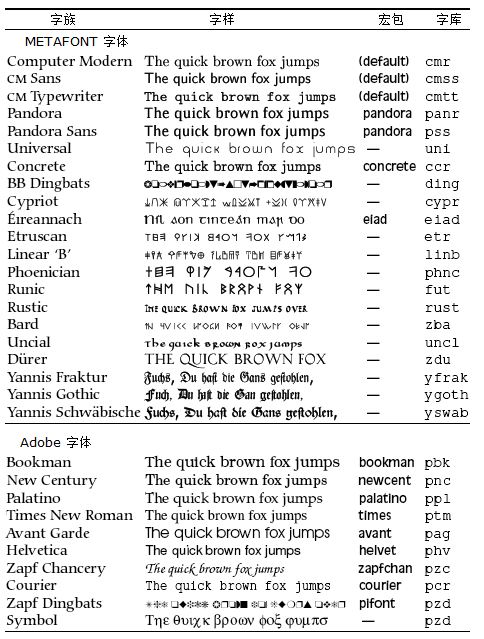
\includegraphics[scale=0.8]{font-1.jpg}
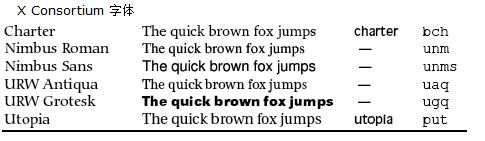
\includegraphics[scale=0.7]{font-2.jpg}
\end{figure}

\section*{NPU-Template}

https://github.com/polossk/LaTeX-Template-For-NPU-Thesis 本科毕设

https://github.com/NWPUMetaphysicsOffice/Yet-Another-LaTeX-Template-for-NPU-Thesis 硕博论文模版持续更新

https://github.com/zhenboliu/npu-PhD-thesis-template  硕博论文

https://github.com/lrtfm/nputhesis  硕博论文

https://github.com/NPUSCG/npu-dissertation-proposal 选题报告

https://github.com/kidozh/LaTeX-Template-For-NPU-Thesis  硕博论文





\end{document}
